%
% teil3.tex -- Beispiel-File für Teil 3
%
% (c) 2020 Prof Dr Andreas Müller, Hochschule Rapperswil
%
% !TEX root = ../../buch.tex
% !TEX encoding = UTF-8
%
\section{Luftwiderstand\label{ueberschall:section:Luftwiderstand}}
\kopfrechts{Luftwiderstand}
Wenige physikalische Phänomene begegnen uns so häufig 
und bleiben dennoch so unsichtbar wie der Luftwiderstand.
Die Berechnung des Luftwiderstandes eines Körpers 
stellt zudem eine der bekanntesten Anwendungen der 
im vorherigen Kapitel behandelten Gleichungen dar.
Besondere Aufmerksamkeit gilt dabei dem Körper mit 
minimalem Wellenwiderstand: 
dem sogenannten Sears-Haack Körper.

\subsection{Analyse des Widerstandsverlaufs}
Wenn wir mithilfe der Strömungsgleichungen den Druckverlauf genauer analysieren, 
lässt sich daraus auch das Verhalten des Luftwiderstands ableiten, 
wie in Abbildung~\ref{fig:luftwiderstand} qualitativ dargestellt.
\begin{figure}
    \centering
    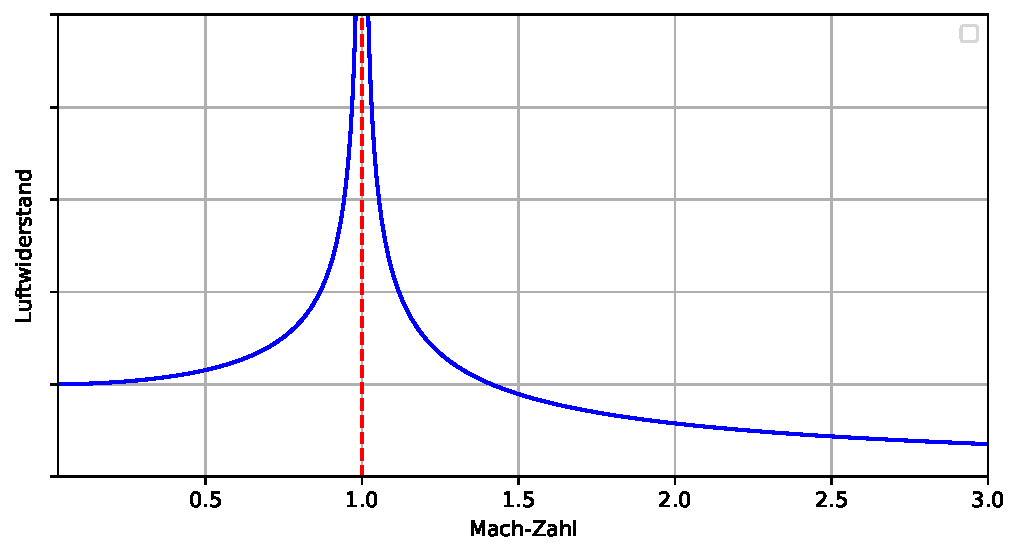
\includegraphics[width=\textwidth]{papers/ueberschall/figures/Luftwiderstand_qual.pdf}
    \caption{Qualitativer Verlauf des Luftwiderstands.}
    \label{fig:luftwiderstand}
\end{figure}
Dabei wird schnell ersichtlich, dass diese theoretische 
Betrachtung nicht der Realität entspricht.
Gemäss den zugrunde liegenden Formeln müsste eine 
unendliche Kraft aufgebracht werden, 
um die Schallgeschwindigkeit zu erreichen — ein Widerspruch zur Tatsache, 
dass moderne zivile Flugzeuge diese Grenze bereits routinemässig überschreiten.

Dies erklärt auch, warum in Abbildung~\ref{fig:abklingen_stromlinie} 
bei Geschwindigkeiten nahe der Schallgeschwindigkeit die Krümmung 
der Stromlinien kaum abklingt.
Es sei daher erneut betont, dass es sich bei den hier 
dargestellten Lösungen um idealisierte Näherungen handelt,
da für die exakte kompressible Strömungsgleichung bislang 
keine geschlossene Lösung bekannt ist 
(vgl. z.\,B. Gleichung~(5) aus~\cite{Ackeret1928}).
Nichtsdestotrotz beschreibt die Näherung das qualitative Verhalten korrekt:
Die Strömungskräfte steigen im Unterschallbereich 
kontinuierlich an und nehmen im Überschallbereich wieder ab.

Zur Veranschaulichung dieses Effekts wird nun ein reales Beispiel 
mit empirisch ermittelten Daten herangezogen:
Ein Projektil des Typs $.50\,\text{BMG}$ M33.
Abbildung~\ref{fig:luftwiderstand_50-M33} zeigt den Verlauf
des Luftwiderstands über der Mach-Zahl.
Dabei ist deutlich zu erkennen, dass der Luftwiderstand 
im Übergang von Unterschall zu Überschall 
deutlich ansteigt und nach dem Überschreiten der 
Schallgeschwindigkeit bei etwa $1{,}2\,\text{Mach}$ 
wieder abnimmt.
Das markante Maximum bleibt bis heute physikalisch 
nicht vollständig erklärbar.
\begin{figure}
    \centering
    \begin{minipage}[t]{0.4\textwidth}
        \centering
        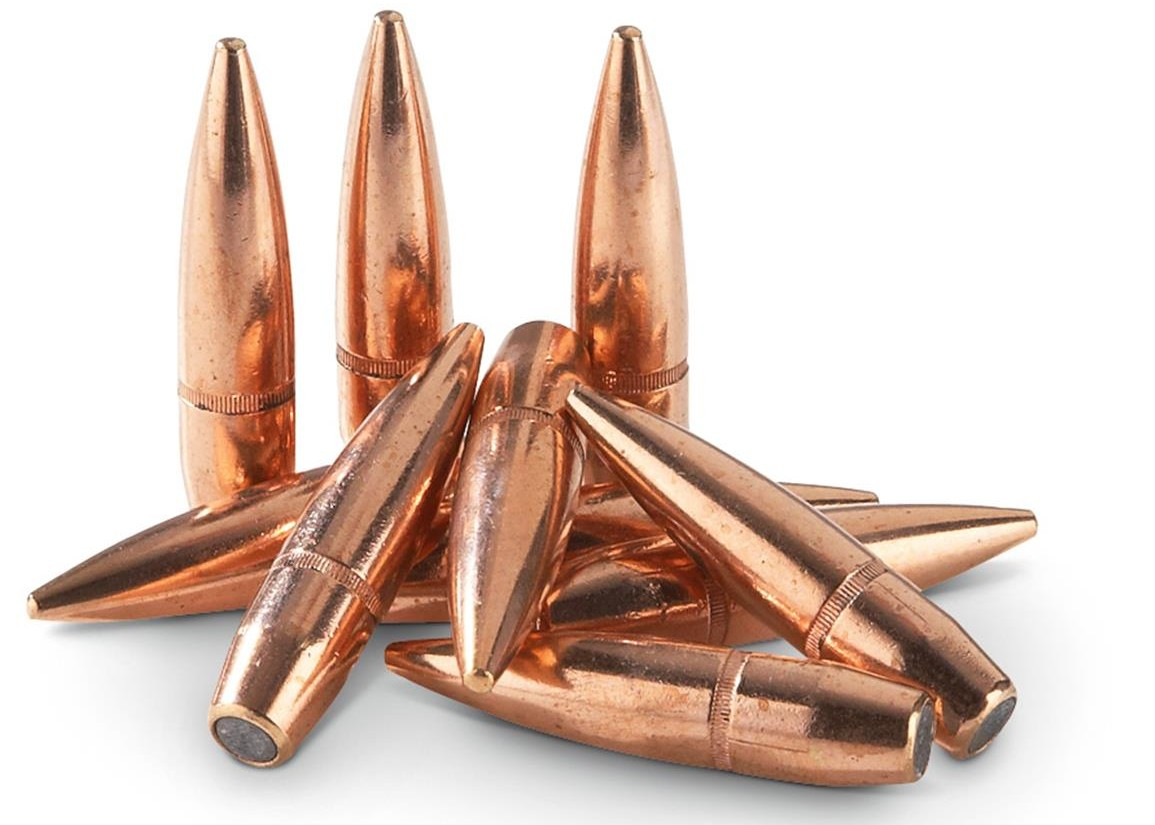
\includegraphics[width=\linewidth]{papers/ueberschall/figures/50-cal_projectile.jpg}
        \caption*{$.50\,\text{BMG}$ M33-Projektil~\cite{ArmoryFarm50BMG}.}
    \end{minipage}
    \hfill
    \begin{minipage}[t]{0.55\textwidth}
        \centering
        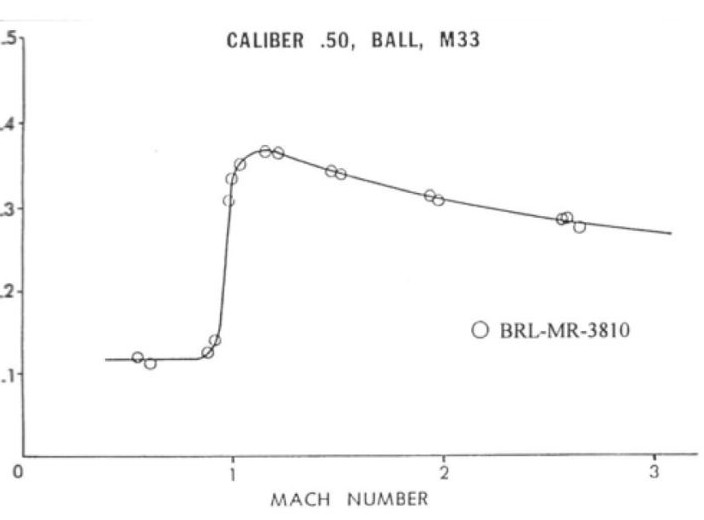
\includegraphics[width=\linewidth]{papers/ueberschall/figures/50-M33 Geschoss.jpg}
        \caption*{Luftwiderstand als Funktion der Machzahl~\cite{Mittelkaliber2020}.}
    \end{minipage}
    \caption{Projektil und Luftwiderstandskurve.}
    ~\label{fig:luftwiderstand_50-M33}
\end{figure}

\subsection{Machsche Kegel}
Es ist zu beachten, dass der Luftwiderstand im Unterschall- und im Überschallbereich 
auf unterschiedlichen physikalischen Mechanismen beruht.
Im Unterschall entsteht der Widerstand hauptsächlich durch die Druckverteilung infolge der Umströmung des Körpers. 
Im Überschall hingegen dominiert der sogenannte Wellenwiderstand, 
dessen Berechnung vergleichsweise einfach ist, 
da er sich aus einer der elementarsten Feldgleichungen 
— der Wellengleichung~\eqref{eq:wellengleichung} — ableiten lässt.

Der Wellenwiderstand entsteht durch das Durchbrechen 
der Schallmauer, wobei ein Teil der Bewegungsenergie 
des Körpers in die Ausbildung von Schockwellen übergeht.
Je nach Form des Objekts kann dieser Anteil deutlich 
geringer sein als der Widerstand im Unterschallbereich.
Ein sichtbares Ergebnis dieser Schockwellen sind die 
sogenannten Machschen Kegel.
An den Schattenbildern der zuvor diskutierten Projektile 
erkennt man deutlich,
wie sich Schockwellen an der Spitze und am Heck 
in Form kegelförmiger Strukturen ausbilden.
\begin{figure}
    \centering
    \begin{minipage}[b]{0.32\textwidth}
        \centering
        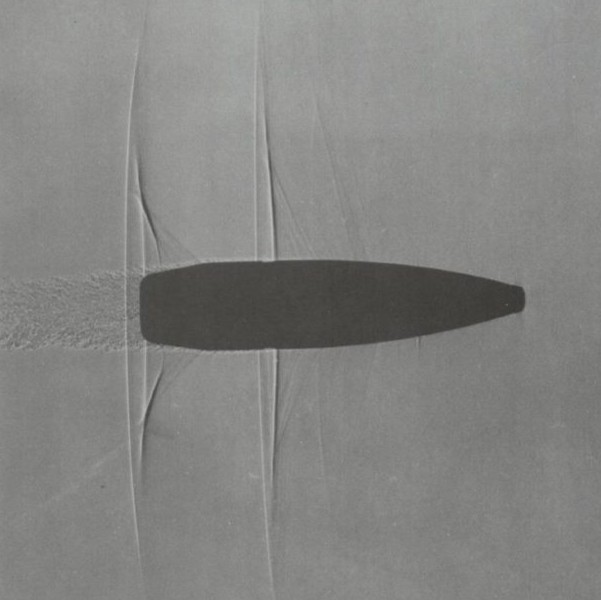
\includegraphics[width=\linewidth]{papers/ueberschall/figures/0.96_mach_projektil.jpg}
        \caption*{$0.96\,\mathrm{Mach}$}
    \end{minipage}
    \hfill
    \begin{minipage}[b]{0.32\textwidth}
        \centering
        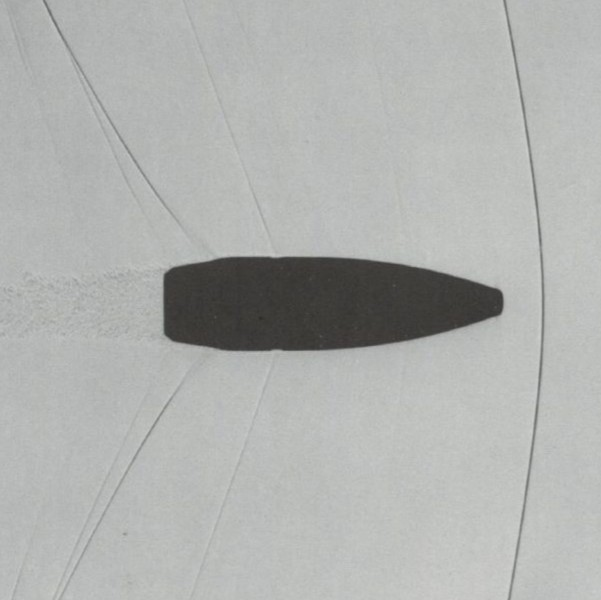
\includegraphics[width=\linewidth]{papers/ueberschall/figures/1.06_mach_projektil.jpg}
        \caption*{$1.06\,\mathrm{Mach}$}
    \end{minipage}
    \hfill
    \begin{minipage}[b]{0.32\textwidth}
        \centering
        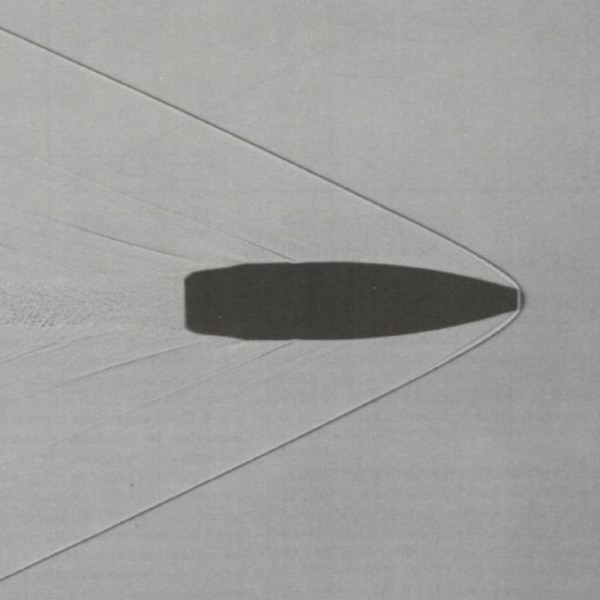
\includegraphics[width=\linewidth]{papers/ueberschall/figures/2.66_mach_projektil.jpg}
        \caption*{$2.66\,\mathrm{Mach}$}
    \end{minipage}
    \caption{Schattenbild von .50 Kaliber M33-Projektile für unterschiedliche Geschwindigkeiten~\cite{Mittelkaliber2020}.}
~\label{fig:machsche_kegel_projektil}
\end{figure}
Man erkennt bereits am ganz links dargestellten Projektil, 
das die Schallgeschwindigkeit noch nicht vollständig 
erreicht hat, die nahezu senkrechten Linien. 
Dies liegt daran, dass die umströmende Luft entlang 
des Projektils schneller ist als das Projektil selbst. 
Dadurch wird lokal die Schallgeschwindigkeit überschritten, 
was zur Ausbildung von Schockwellen führt.

Gut erkennbar ist, wie der Winkel des dadurch entstehenden 
Kegels von der Geschwindigkeit des Profils abhängt. 
Dieser Winkel wird als Mach-Doppler-Winkel $\alpha$ 
bezeichnet und ist durch die folgende Beziehung gegeben:
\begin{align*}
      \tan \alpha 
      = 
      \frac{1}{\sqrt{\frac{U^2}{a^2} - 1}},
\end{align*}
wobei $U$ die Geschwindigkeit des Objekts und $a$ 
die Schallgeschwindigkeit in der umströmenden Luft 
bezeichnet. 
Daraus folgt unmittelbar
\begin{align*}
      \sin \alpha 
      = 
      \frac{\tan \alpha}{\sqrt{1 + \tan^2 \alpha}} 
      = 
      \frac{a}{U}.
\end{align*}
Aufgrund dieser Zusammenhänge kann aus einem Schattenbild 
die Geschwindigkeit eines Objekts im Überschallbereich 
bestimmt werden.

\subsection{Sears-Haack Körper}
Die Minimierung des Luftwiderstands im Überschallbereich 
gestaltet sich deutlich einfacher als im Unterschall. 
Einen Körper zu finden, der sowohl im Unterschall-, 
transsonischen als auch im Überschallbereich optimal ist, 
erweist sich aufgrund der unterschiedlichen 
Strömungsmechaniken als kaum möglich.
Daher beschränken wir uns im Folgenden auf den einfachsten Fall.
Der Sears-Haack Körper, illustriert in Abbildung~\ref{fig:sears_haack} 
besitzt den theoretisch geringsten Wellenwiderstand. 
Im Bereich von etwa $1{,}5$ bis $3\,\mathrm{Mach}$ 
stellt er die strömungsgünstigste Form dar. 
Wolfgang Haack bestimmte diese Form mithilfe des 
Variationsprinzips und legte die ausführliche Herleitung 
in~\cite{Haack1941} vor.
\begin{figure}
    \centering
    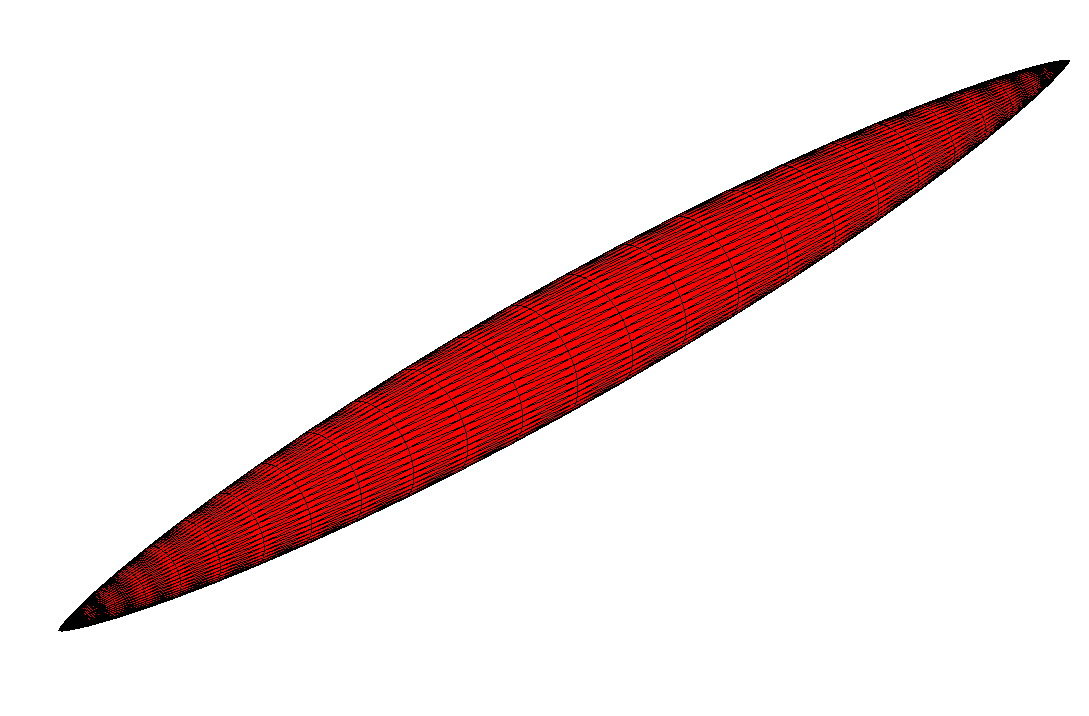
\includegraphics[width=0.6\textwidth]{papers/ueberschall/figures/Sears-Haack.png}
    \caption{Der Sears-Haack Körper~\cite{SearsHaackWikipedia}.}
    \label{fig:sears_haack}
\end{figure}

Haacks ursprüngliches Ziel war die Optimierung von Scharfschützengewehren. 
Praktische Gründe führten jedoch dazu, dass diese 
Form nicht verwendet wurde. 
Stattdessen erfolgte die Optimierung der Projektile 
durch einen Heckkonus, wie in Abbildung~\ref{fig:luftwiderstand_50-M33} dargestellt.
Nichtsdestotrotz hat der Sears-Haack Körper aufgrund 
seiner strömungsoptimierten Form eine große Bedeutung 
für die Gestaltung von Flugkörpern und Raketen im 
Überschallbereich erlangt.


 